\section{Versuchsaufbau}

Für den Versuch wird ein Gerüst benutzt, dass einem glatetn Brett ermöglicht den Winkel mit der horizontalen Ebene einzustellen. An beiden Enden des Bretts befindet sich jeweils eine verschiebbare Lichtschranke.\\
Ein Holzquader mit vier unterschiedlichen Oberflächen wird auf das glatte Brett gelegt. Eine Seite des Quaders ist unbeschichtet, eine ist mit Gummi beklebt, auf einer ist Klebeband und die letzte Seite ist lackiert. Der Quader rutscht über das Brett, sobald der Winkel hoch genug ist.\\
Ebenfalls wird ein Gliedermaßstab gebraucht, um die Länge $l$ zwischen den Lichtschranken zu messen, und ein Winkelmesser, mit dem $\alpha$ berechnet wird.
\begin{figure}[ht]
    \centering
    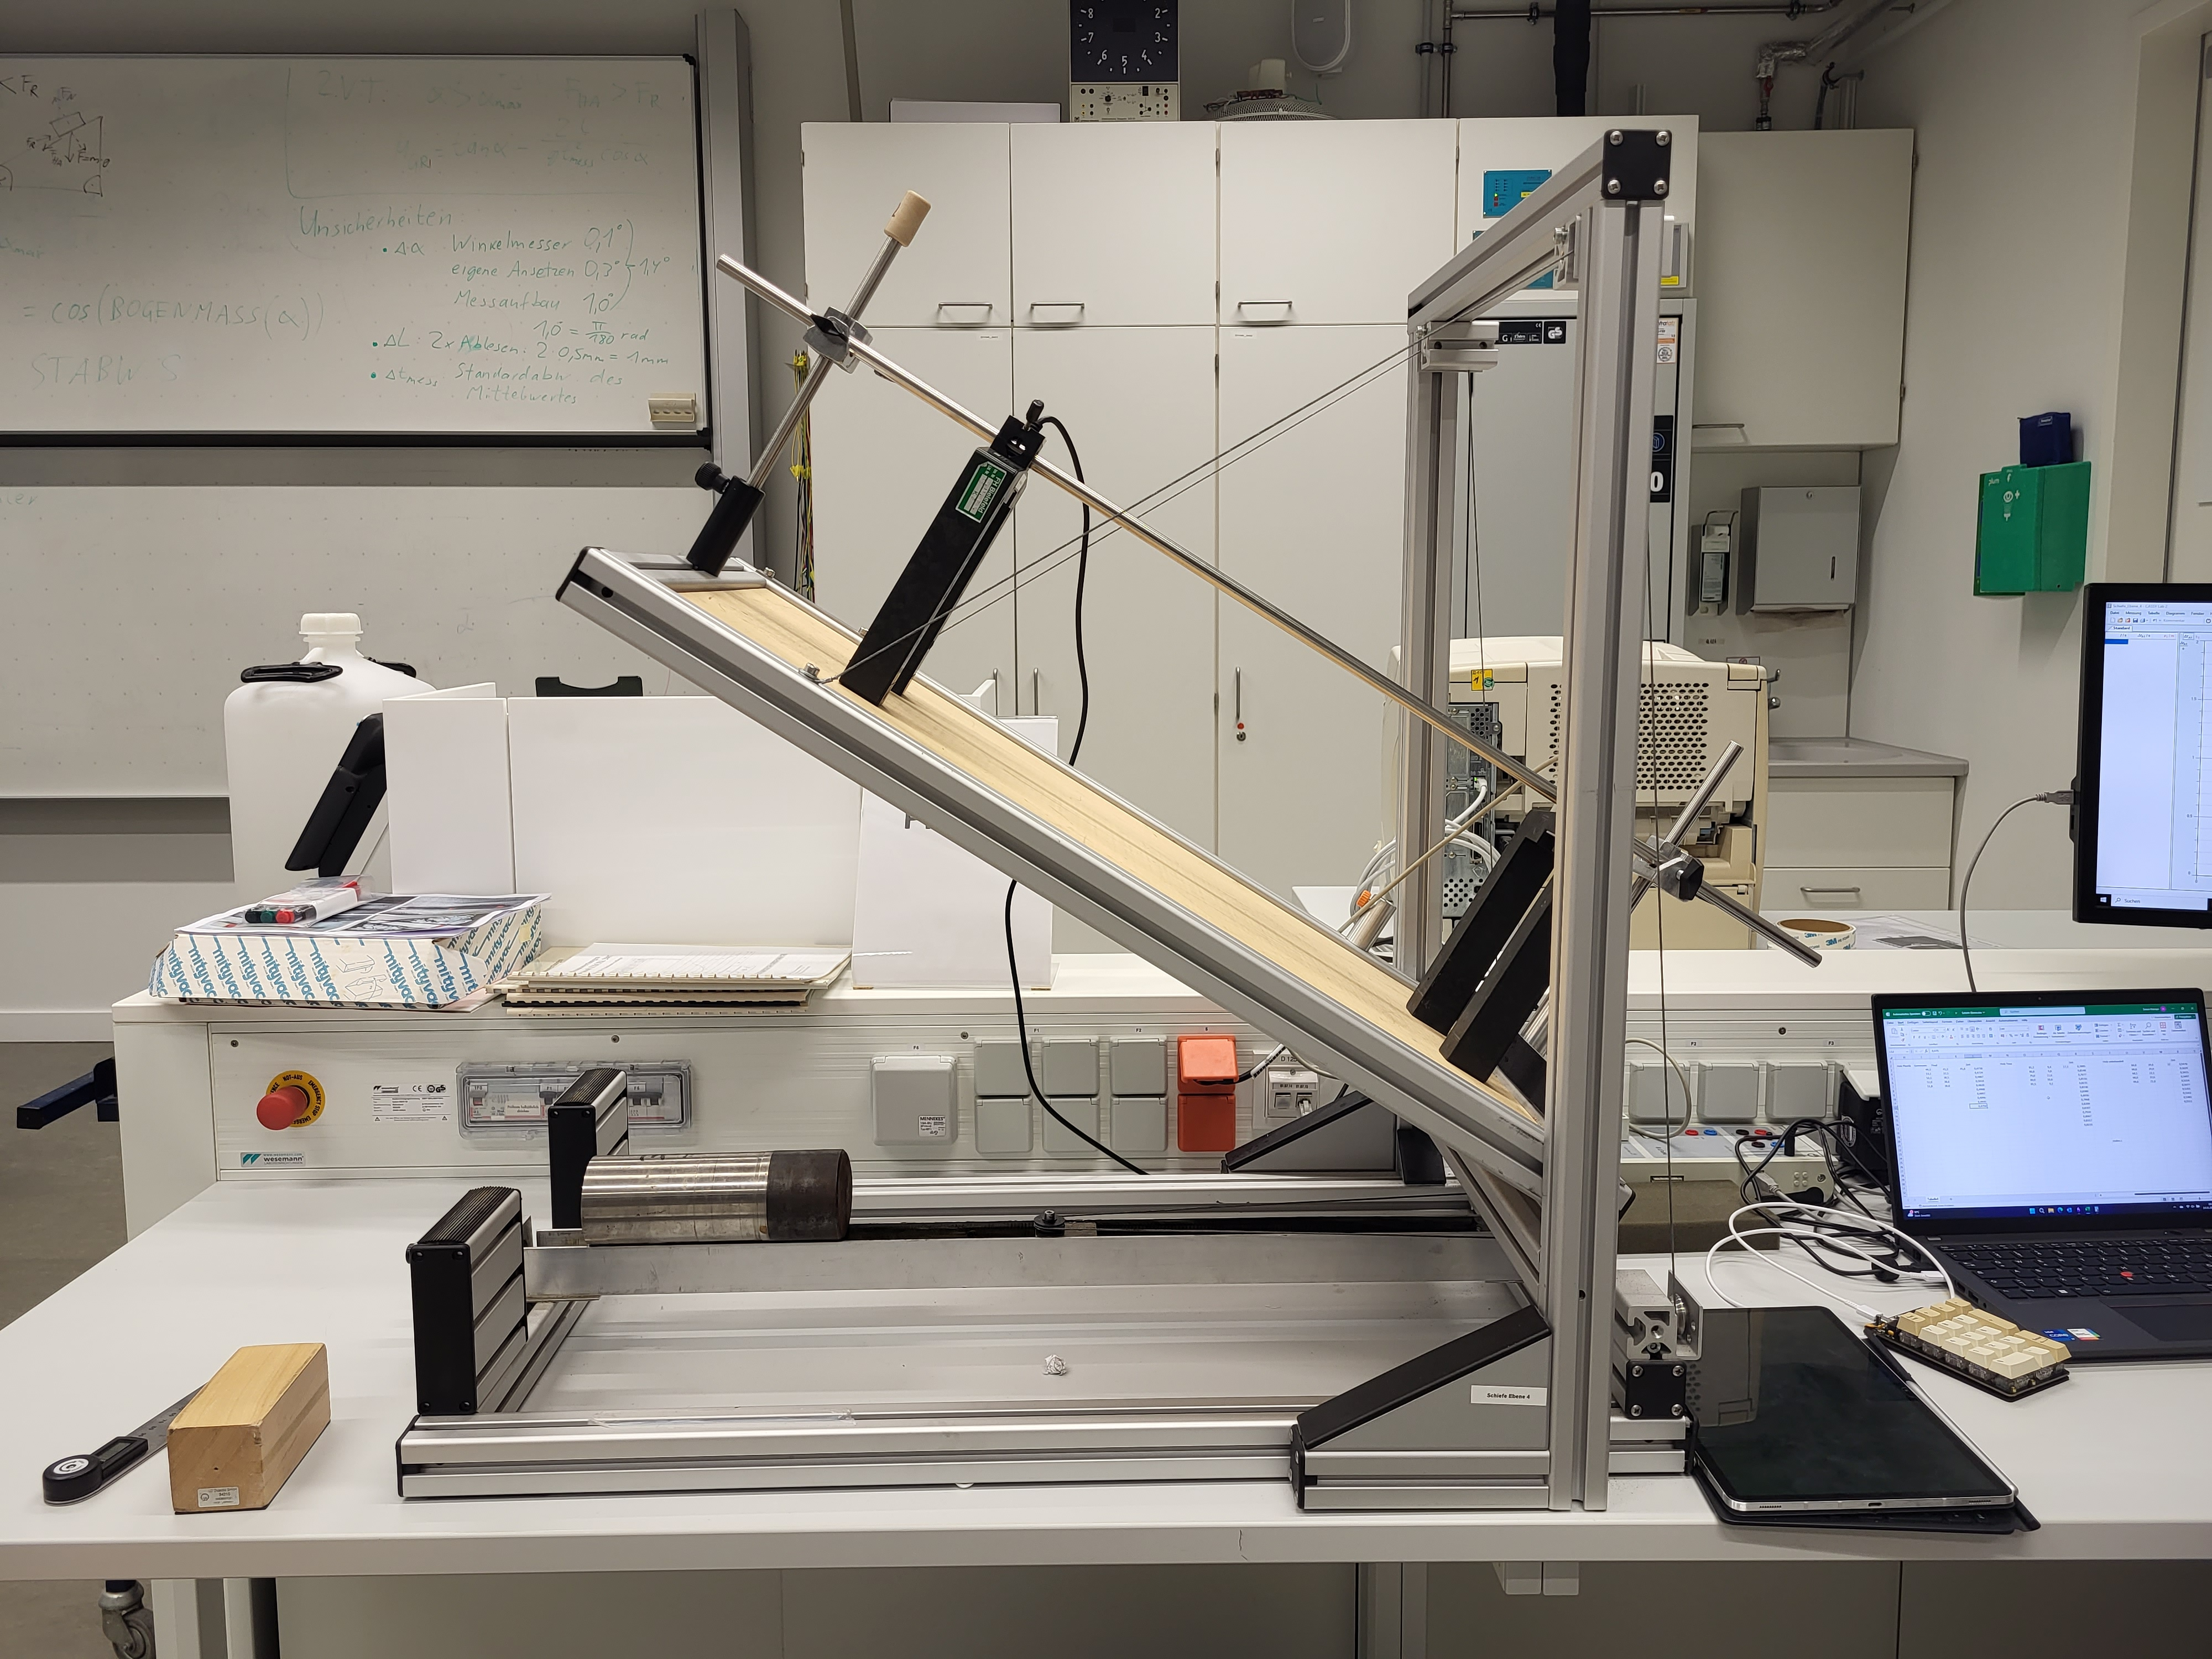
\includegraphics[width=\linewidth/2]{images/Versuch-Aufbau.jpg}
    \caption[Aufbau]{Gerüst mit glattem Brett und Lichtschranken}
    \label{fig:Aufbau}
\end{figure}